\documentclass{beamer}

\usepackage{lmodern}
\usepackage[frenchb]{babel}
\usepackage[T1]{fontenc}
\usepackage[utf8]{inputenc}
\usepackage{graphicx}
\usepackage{wrapfig}

\usetheme{Warsaw}

\setbeamertemplate{footline}[frame number]

% metadata
\title{Informatique et programmation dans les nuages (cloud)}
\author{Jules Lamur, Denis Hodzhadzhikov}
\institute{Université de Montpellier 2}
\date{13 mars 2017}

\AtBeginSubsection[]
{
\begin{frame}<beamer>{Sommaire}
    \tableofcontents[currentsection,currentsubsection]
\end{frame}
}

\begin{document}

\begin{frame}
    \titlepage
\end{frame}

\begin{frame}
    \tableofcontents
\end{frame}

\section{C'est quoi le cloud ?}
\pause
\begin{frame}{C'est quoi le cloud ?}
    \centerline{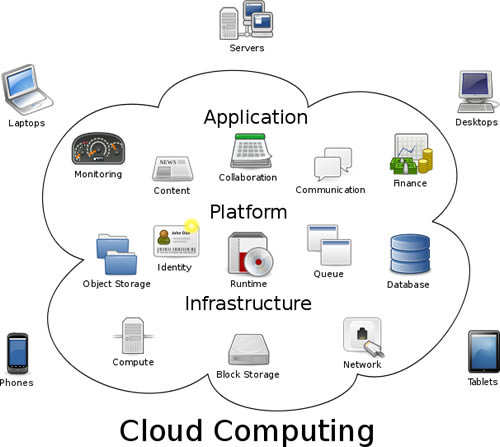
\includegraphics[width=0.75\textwidth]{images/cloud_computing.jpg}}
\end{frame}

\subsection{Définition}

\begin{frame}{Définition}
    \begin{block}{Définition}
        Le cloud computing est un concept qui représente \textbf{l’accès à des informations et services, situés sur un serveur distant}.
    \end{block}
    \pause
    Autrement dit, il s’agit d’une forme d’externalisation des serveurs et services rattachés d’une entreprise donnée.
\end{frame}

\subsection{Historique}

\begin{frame}{Historique}
    \begin{itemize}
        \item {
        Un principe vieux comme l'informatique (1950).
        }\pause
        \item {
        Qui connait une croissance exponentielle depuis les années 2000.
        Notamment chez les entreprises très gourmandes en services délocalisés (exemples : messagerie, fichiers, logiciels de gestion).
        }\pause
        \item {
        L'arrivée du haut debit a joué un rôle important dans l'adoption du cloud.
        }
    \end{itemize}
\end{frame}

\section{Les services}

\subsection{Les différents types de service}

\begin{frame}{Les différents types de service}
    \begin{figure}[h]
        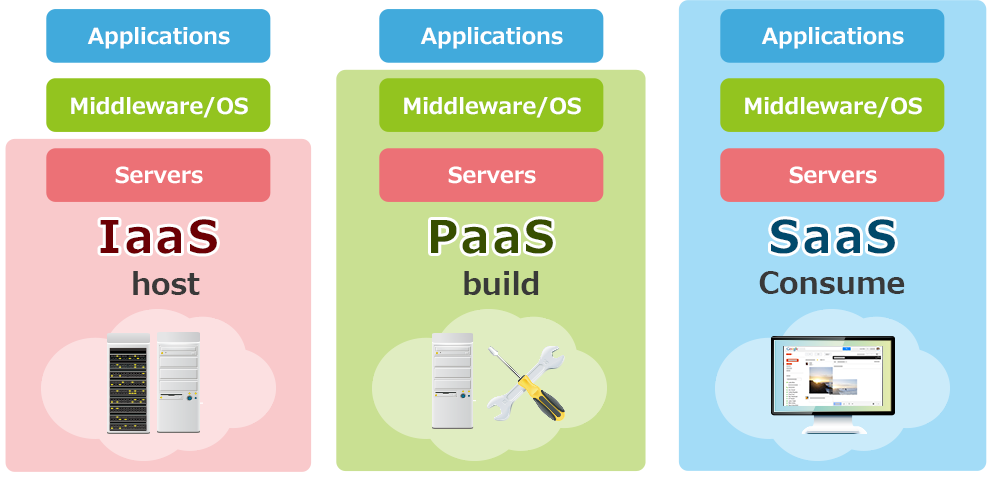
\includegraphics[width=\textwidth]{images/services.png}
    \end{figure}

    Il en existe beaucoup d'autres.
\end{frame}

\subsection{Infrastructure as a Service (IaaS)}

\begin{frame}{Infrastructure as a Service (IaaS)}
    \begin{wrapfigure}{r}{0.30\textwidth}
        \centering
        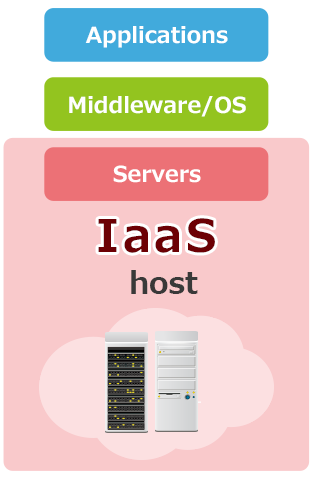
\includegraphics[width=0.30\textwidth]{images/services_iaas.png}
    \end{wrapfigure}

    L'IaaS donne accès aux ressources informatiques dans un environnement virtualisé :
    \pause

    \begin{itemize}
        \item {
        Le fournisseur gère le matériel serveur, le stockage, le réseau.
        }\pause
        \item {
        Le client gère le middleware des serveurs, et surtout les logiciels applicatifs.
        }\pause
        \item {
        De très nombreux fournisseurs existent, on peut citer par exemple :
        Amazon EC2, OVH Instance, VMware Dedicated Cloud.
        }
    \end{itemize}
\end{frame}

\subsection{Platform as a Service (PaaS)}

\begin{frame}{Platform as a Service (PaaS)}
    \begin{wrapfigure}{r}{0.30\textwidth}
        \centering
        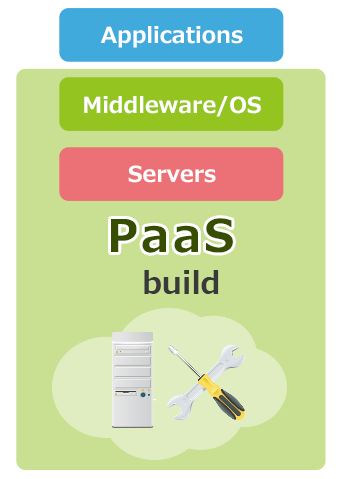
\includegraphics[width=0.30\textwidth]{images/services_paas.png}
    \end{wrapfigure}

    Les services PaaS font abstraction du middleware pour permettre une installation
    et un déploiement simplifié des applications.
    \pause

    \begin{itemize}
        \item {
        Le fournisseur gère (comme pour l'IaaS) le matériel serveur, le stockage, le réseau.
        Il gère également le système d'exploitation et les services dépendants des applications.
        }\pause
        \item {
        L'hébergement web mutualisé en est un bon exemple. Le fournisseur gère les serveurs HTTP,
        SQL et FTP et le client, le code source de l'application.
        }
    \end{itemize}
\end{frame}

\subsection{Software as a Service (SaaS)}

\begin{frame}{Software as a Service (SaaS)}
    \begin{wrapfigure}{r}{0.30\textwidth}
        \centering
        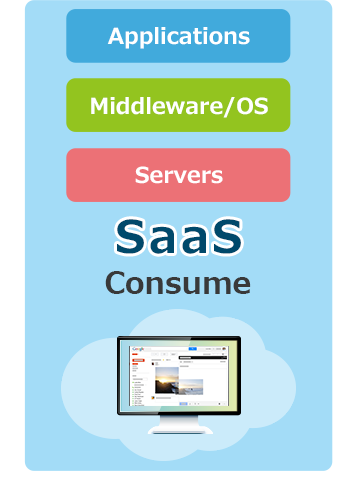
\includegraphics[width=0.30\textwidth]{images/services_saas.png}
    \end{wrapfigure}

    Le SaaS est très utilisé chez les particuliers et les entreprises car il
    demande peu ou aucune connaissance technique dans la mise en place.
    \pause

    \begin{itemize}
        \item {
        Ses applications sont nombreuses (messagerie, gestionnaire de relation client,
        communication, site internet clés-en-main).
        }\pause
        \item {
        Le client n'achète pas de licence, mais paye un abonnement
        pour utiliser le service en ligne.
        }
    \end{itemize}
\end{frame}

\section{L'infrastructure}

\subsection{Serveur dédié}

\begin{frame}{Serveur dédié}
    \begin{itemize}
        \item {
        Méthode "classique".
        }\pause
        \item {
        Accès direct aux resources hardwares : meilleures performances.
        }\pause
        \item {
        Difficile à faire évoluer.
        }\pause
        \item {
        Non scalable à l'échelle d'une machine.
        }\pause
        \item {
        Au final, installation et gestion complexe pour les grosses infrastructures.
        }
    \end{itemize}
\end{frame}

\subsection{Virtualisation et pooling}

\begin{frame}{Virtualisation et pooling}
    \begin{block}{Virtualisation}
        \pause
        Faire fonctionner un système d'exploitation comme un simple logiciel.
        Le système ainsi créé s'appelle \textbf{une machine virtuelle}.
    \end{block}
    \pause
    \begin{block}{Pooling}
        \pause
        Mise en commun des resources de plusieurs machines physiques pour y
        déployer des machines virtuelles interconnectées.
    \end{block}
\end{frame}

\begin{frame}{Virtualisation et pooling}
    \begin{itemize}
        \item {
        Repose sur une installation de serveurs en réseau.
        }\pause
        \item {
        Offre une très grande souplesse d'évolution.
        }\pause
        \item {
        Scaling vertical et horizontal simplifié.
        }\pause
        \item {
        Performances moins bonnes qu'un serveur dédié.
        }\pause
    \end{itemize}
\end{frame}

\begin{frame}{OpenStack}
    \begin{figure}[h]
        
\includegraphics[width=0.30\textwidth]{images/openstack-logo.png}
    \end{figure}
    \textbf{OpenStack} est un ensemble de logiciels open source permettant de déployer des infrastructures de cloud computing (IaaS).
\end{frame}

\begin{frame}{OpenStack}
    \begin{itemize}
        \item {
        Initialement développé par la \textit{NASA} et \textit{Rackspace Hosting}.
        }\pause
        \item {
        Open source, maintenu par plus de 150 grandes entreprises dans le monde.
        }\pause
        \item {
        Utilisé par des milliers d'entreprises dans divers secteurs d'activité (finances, commerce, télécom, énergie, recherche, etc..).
        }\pause
    \end{itemize}
\end{frame}

\begin{frame}{OpenStack}
    Fonctionne sous forme de \textit{briques} implémentant différentes fonctionnalités :
    \pause
    \begin{itemize}
        \item {
        Stockage (\textit{Swift}),
        }\pause
        \item {
        Calcul (\textit{Nova}),
        }\pause
        \item {
        Réseau (\textit{Neutron}),
        }\pause
        \item {
        Webinterface de gestion (\textit{Horizon}),
        }\pause
        \item {
        Et biens d'autres (19 au total).
        }\pause
    \end{itemize}
\end{frame}

\begin{frame}{OpenStack}
    Exemple d'architecture simple avec 4 briques (calcul, réseau, stockage, webinterface) :
    \begin{figure}[h]
        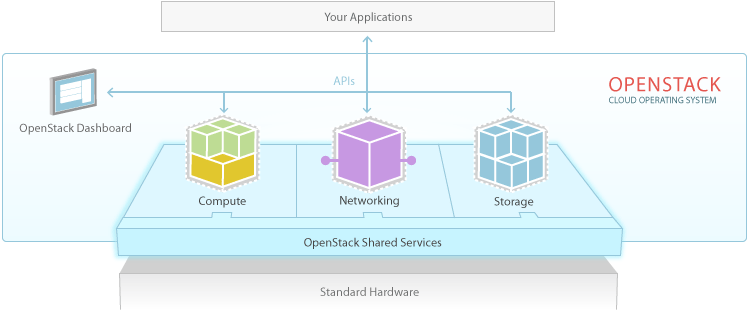
\includegraphics[width=\textwidth]{images/openstack-software-diagram.png}
    \end{figure}
\end{frame}

\section{Conclusion}

\begin{frame}{Avantages}
    \begin{itemize}
        \pause
        \item {
        Haute scalabilité.
        }\pause
        \item {
        Permet de combiner des ressources hétérogènes (matériel, logiciel, trafic réseau).
        }\pause
        \item {
        Accessibilité facile aux differents données à tout moment, n'importe où et sur tous les supports.
        }\pause
        \item {
        Pas nécessaire de dépenser beaucoup d'argent sur le matériel, les logiciels ou les droits de licence  (\textit{Pay as you go}).
        }
    \end{itemize}
\end{frame}

\begin{frame}{Inconvénients}
    \begin{itemize}
        \pause
        \item {
        Risques de sécurité.
        }\pause
        \item {
        Problèmes techniques.
        }\pause
        \item {
        Connexion nécessaire.
        }
    \end{itemize}
\end{frame}

\begin{frame}{Fin}
    \centerline{
\includegraphics[width=0.5\textwidth]{images/fin.jpg}}
\end{frame}

\begin{frame}{Bibliographie}
    \begin{thebibliography}{2}
        \bibitem{}
        https://fr.wikipedia.org/wiki/Cloud\_computing
        \bibitem{}
        https://www.openstack.org
    \end{thebibliography}
\end{frame}



\end{document}
